\documentclass[11pt, a4paper, titlepage, twoside]{article}

\usepackage[utf8]{inputenc}
\usepackage[T1]{fontenc}
\usepackage[french]{babel}

\renewcommand{\emph}{\textbf}
\usepackage{cmbright}

\usepackage[a4paper, left=3cm, right=3cm, top=3.5cm, bottom=3.5cm]{geometry}
\usepackage[automark, headsepline, footsepline]{scrpage2}
\usepackage{indentfirst}
\usepackage{graphicx}
\usepackage[labelfont=bf, textfont=it]{caption}
\usepackage{setspace}
\usepackage[nottoc]{tocbibind}

\newcommand{\version}{1.2.1}

\usepackage[
	pdftitle = {SortSimulation},
	pdfsubject = {Dokumentation},
	pdfauthor = {Peter\ {}Folta},
	pdfkeywords = {},
	pdfcreator = {},
	pdfproducer = {},
	colorlinks = true,
	linkcolor = black,
	anchorcolor = black,
	citecolor = black,
	filecolor = black,
	menucolor = black,
	pagecolor = black,
	urlcolor = blue]{hyperref}

\usepackage{listings}
\renewcommand{\lstlistingname}{Listing}
\renewcommand{\lstlistlistingname}{Listings}
\lstset{basicstyle=\ttfamily, tabsize=4, numbers=left, numberstyle=\scriptsize, xleftmargin=20pt}

\title{SortSimulation}
\author{Peter Folta}

\clearscrheadfoot
\ihead[\headmark]{\headmark}
\ohead[\pagemark]{\pagemark}
\ifoot[SortSimulation~-- Documentation]{SortSimulation~-- Documentation}
\ofoot[Version \version]{Version \version}

\pagestyle{scrheadings}

\onehalfspacing

\begin{document}
	\pagenumbering{roman}
	
	\begin{titlepage}
		\begin{center}
			\vspace*{2.5cm}
			\Huge{\textbf{SortSimulation}}
			
			\vspace*{1.5cm}
			\LARGE{Documentation}
			
			\Large{-- Français --}
			
			\vspace*{3.75cm}
			\Large{Peter Folta}
		\end{center}
		
		\vspace*{8cm}
		\noindent{}Version \version\newline{}
		Site Web: \href{http://www.peterfolta.de/software/sortsimulation}{http://www.peterfolta.de/software/sortsimulation}\newline{}
		Copyright \textcopyright{} 2008--2009 Peter Folta. Tous droits réservés.
	\end{titlepage}
	
	\setcounter{page}{2}
	
	\cleardoublepage{}
	\tableofcontents{}
	\newpage{}
	
	\pagenumbering{arabic}
	
	\section{Introduction}
	
	SortSimulation est un programme java que visualise des méthodes de tri. D’un coté on peut mieux comprendre mieux le mode de fonctionnement des algorithme de tri et de l’autre le programme explique les différence en ce qui se concerne les périodes d'action sans comparer des chiffres.
	
	\begin{figure}[h]
		\begin{center}
			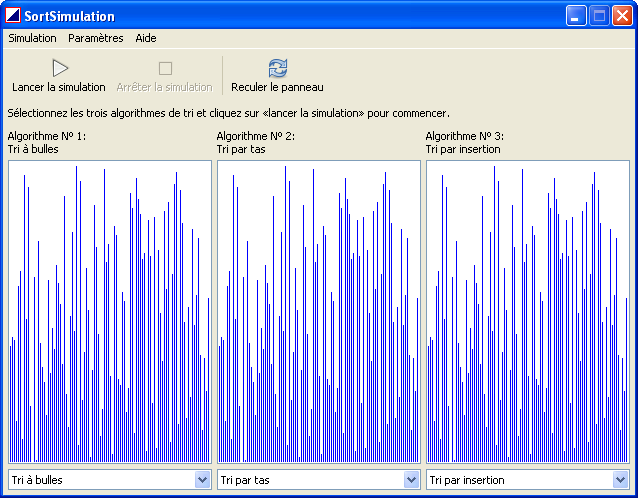
\includegraphics[scale=0.6]{images/image0.png}
			\caption{La fenêtre principale de SortSimulation}
		\end{center}
	\end{figure}
	
	Ce document consiste d’une introduction courte concernant la commande et une présentation des méthodes de tri soutenu, le mise en œuvre de Java inclus.
	
	\section{Commande}
	
	La commande de SortSimulation est simple: Après le lancement du programme les panneau de tri sont de déjà remplies par hasard. Dans touts les panneau il y a la même situation de base. En outre trois méthodes de tri sont déjà ajustés, on peut voir cela á cause de liste déroulante au dessous des panneaux.
	
	Alors pour comparer les trois algorithmes de tri, il faut choisir les méthodes dans les listes déroulantes. La simulation lance dés que vous avez cliqué sur le bouton de commande \emph{Lancer la simulation} au barre d'outils, après vous avez choisi l'entrée correspondant dans le menu ou pressé la touche d'entrée. Pour arrêter une simulation courante il faut presser la touche Échappement ou on peut clique sur le bouton \emph{Arrêter la simulation}. Pour obtenir après une simulation arrêtée ou finie des panneaux non assorti, cliquez sur le bouton \emph{Reculer le panneau} ou pressez \texttt{Ctrl+N}.
	
	SortSimulation vous offre plusieurs paramètres pour adapter la simulation. Dans le paragraphe suivant les paramètres sont expliqués détaillés.
	
	\subsection{Paramètres}
	
	Plusieurs paramètres sont á votre disposition chez SortSimulation pour ajuster la simulation de tri comme vous voulez. Vous trouvez les possibilités d'ajuster dans le menu \emph{Paramètres}:
	
	\begin{figure}[h]
		\begin{center}
			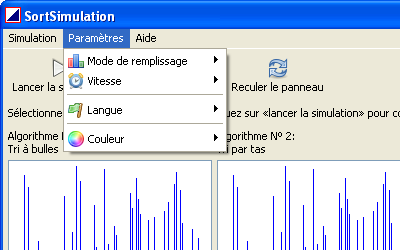
\includegraphics[scale=0.6]{images/image1.png}
			\caption{Menu «\,Paramètres\,»}
		\end{center}
	\end{figure}
	
	L'option \emph{Mode de remplissage} vous offre la possibilité de choisir la sorte de remplissage quand l'action \emph{Reculer le panneau} s'est déroule. Il y a deux modes pour cet action: par hasard (présélectionné; \texttt{Ctrl+R}) et l'inverse (\texttt{Ctrl+I}). Dans le mode \emph{Par hasard} les éléments sont arrangés  par hasard á chaque remplissage du panneau de sorte qu'on puisse essayer réalistement des méthodes de tri avec des dates non sortie.
	
	Dans le mode \emph{Inverse} au contrarie les panneau sont déjà rempliés mais à l'envers (décroissant au lieu de ascendant) pour savoir l'efficience les méthodes de tri concernant les séquences qui sont sorties à l'envers.
	
	Le sous-menu \emph{Vitesse} vous donnez la possibilité de choisir la vitesse. Vous avez le choix entre cinq degrés. Pendant que les algorithmes comme tri à bulles sont très lente et ainsi une grande vitesse s'offre, il est profitable de regarder par exemple tri rapide lentement pour pouvoir comprendre le fonction. La vitesse se laisse aussi controler par la combinaison de ouches \texttt{Ctrl+Shift+(1-5)}.
	
	SortSimulation n'écrit pas des données sur votre ordinateur ou les modifies, à cause de cela le programme commence chaque fois avec une interface anglais. Vous pouvez changer le langue dans le menu (anglais: \emph{Settings} > \emph{Language}).
	
	Dans le sous-menu \emph{Couleur} vous pouvez ajuster le couleur des barres. Le standard est bleu mais vous avez le choix entre huit couleur.
	
	\section{Méthodes de tri}
	
	\subsection{Tri à bulles}
	
	Tri à bulles est un algorithme de tri simple que sort les éléments en comparant \emph{par étapes}. Tri à bulles n'est pas efficace ainsi on utilise l'algorithme pour démontrer un mauvais méthode de tri.
	
	\subsubsection{L'idée de tri à bulles}
	
	Tri à bulles compare deux élément voisin et les change si l'ordre  n'est pas correct. Cet action se repasse jusqu'à toutes les éléments sont en bon ordre c'est-à-dire qu'il sont sortis.
	
	\subsubsection{Mise en œuvre de Java}
	
	\lstinputlisting[caption={Mise en oeuvre de tri à bulles}, label=lst:bubblesort, captionpos=b]{../Listings/Bubblesort.java}
	
	\subsection{Tri par tas}
	
	Tri par tas est un méthode de tri vite que c'était inventé par \emph{Robert W Floyd} et \emph{J.\,W.\,J.\,Williams} en 1964 sur la base de \emph{tri par sélection}.
	
	\subsubsection{L'idée de tri par tas}
	
	Tri par tas utilise pour le triage une structure des données particulière; le \emph{tas} qui est fondé sur un arbre qui est presque totalement binaire. Un arbre binaire est (presque) complet quand toutes les  plans sauf éventuellement la dernière sont complètes.
	
	Quand on a une séquence tas, le plus grand élément de la \emph{racine} d'arbre peut être échantillonné et distribué. Pour avoir accès au élément supérieur, il faut \emph{ordre le tas à nouveau}.
	
	\subsubsection{Mise en œuvre de Java}
	
	\lstinputlisting[caption={Mise en oeuvre de tri par tas}, label=lst:heapsort, captionpos=b]{../Listings/Heapsort.java}
	
	\subsection{Tri par insertion}
	
	Tri par insertion est une méthode de tri simple qui n'est pas si efficace comme des algorithmes plus complexes, mais on peut la mettre plus \emph{facilement en œuvre} et elle a besoin d'une distance électrique courte quand on a peu des données ou quand ils sont déjà tris.
	
	\subsubsection{L'idée de tri par insertion}
	
	Tri par insertion échantillonne une élement d'une ensemble non tri et l'ajoute à la vraie position dans la séquence de distribution. Si la séquence est encore vide, l'élément est collée à la première position.
	
	Tri par insertion n'est pas efficace car cette méthode de tri doit délocaliser les éléments souvent par des distances vaste.
	
	\subsubsection{Mise en œuvre de Java}
	
	\lstinputlisting[caption={Mise en oeuvre de tri par insertion}, label=lst:insertionsort, captionpos=b]{../Listings/Insertionsort.java}
	
	\subsection{Tri fusion}
	
	Tri fusion est un algorithme de tri récursif et stable qui base sur le principe \emph{Divide-and-Conquer}. Tri fusion était présenté en 1945 par John von Neumann.
	
	\subsubsection{L'idée de tri fusion}
	
	Tri fusion décompose la séquence en plusieures petites séquences qui sont triés isolements. Puis les petites séquences sont assemblées selon le principe de la fermeture éclair jusqu'au moment quand toutes les éléments sont triés pour avoir une grande séquence.
	
	\subsubsection{Mise en œuvre de Java}
	
	\lstinputlisting[caption={Mise en oeuvre de tri fusion}, label=lst:mergesort, captionpos=b]{../Listings/Mergesort.java}
	
	\subsection{Tri rapide}
	
	Tri rapide est une des méthodes de tri \emph{les plus rapides} qui base sur le principe \emph{Divide-and-Conquer}. En 1960 la version initial de l'algorithme récursif de tri rapide était développé par \emph{C. Antony R. Hoare}.
	
	\subsubsection{L'idée de tri rapide}
	
	La séquence qu'on veut trier est d'abord fragmenté en deux parts afin que les éléments dans la première fragment sont plus petites ou égaux que les élément dans la deuxième fragment (\emph{divide}). Puis les deux fragment sont triés isolements dans une manière récursive en utilisant la même méthode (\emph{conquer}). Dans le dernier étape les fragments assemblées donnent la séquences triée (\emph{combine}).
	
	La partition est réalisé  à l'aide d'un \emph{élément pivot} qui est choisi pendant la première étape de la séquence. Toutes les éléments de la séquence qui sont \emph{plus petites} que l'élément pivot, viennent au première tronçon. Toutes les éléments qui sont \emph{plus grandes} que l'élément pivot au deuxième tronçon. En ce qui se concerne les éléments qui sont autant grandes que l'élément pivot il ne joue aucun rôle d'où ils viennet.
	
	\subsubsection{Mise en œuvre de Java}
	
	\lstinputlisting[caption={Mise en oeuvre de tri rapide}, label=lst:quicksort, captionpos=b]{../Listings/Quicksort.java}
	
	\subsection{Tri par sélection}
	
	Tri par sélection est un algorithme de tri naïve qui travaille sur place.
	
	\subsubsection{L'idée de tri par sélection}
	
	Tri par sélection fragmente la séquence de tri en un part \emph{trié} et un part \emph{non-trié}. Au début le part trié est vide. Tri par sélection cherche le plus petit élément dans le part non-trié et le remplace avec le première élément. Après cela la séquence est triée jusqu'à cette position. Le part trié a grandi par un élément, le part non-trié a diminué par un élément. La méthode est répété jusqu'au moment quand la séquences est triée complètement.
	
	\subsubsection{Mise en œuvre de Java}
	
	\lstinputlisting[caption={Mise en oeuvre de tri par sélection}, label=lst:selectionsort, captionpos=b]{../Listings/Selectionsort.java}
	
	\subsection{Tri de Shell}
	
	Tri de Shell est une méthodes de tri qui est basé sur \emph{tri par insertion}. Tri de Shell était développé par \emph{Donald L. Shell} en 1959.
	
	\subsubsection{L'idée de tri de Shell}
	
	Tri de Shell compense le désavantage d'tri de insertion, les éléments ne doivent plus être déplacés par des distances longues. Pour réaliser cela, tri de Shell produit une \emph{matrice k-délitescente}, les colonnes du matrice sont triés isolements. Après cela la séquence est déjà triée bourrue. Cette démarche est répétée, le nombre des colonnes se réduit pendant chaque réalisation jusqu'au moment quand il y a seulement une colonne.
	
	\subsubsection{Mise en œuvre de Java}
	
	\lstinputlisting[caption={Mise en oeuvre de tri de Shell}, label=lst:shellsort, captionpos=b]{../Listings/Shellsort.java}
	
	\section{Coopérateurs}
	
	Je remerie les personnes suivantes qui m'a soutenu allantement de développer SortSimulation. Des nouveaux coopérateurs (traducteurs, designer, auteurs des documentations, etc.) sont cherchés continuellement. Si vous avez envie de soutenir les projets de Peter Folta, contactez -le.
	
	\subsection{Traducteurs}
	
	\begin{itemize}
		\item{Folta, Lucia Sonja~-- Russe}
		\item{Folta, Peter~-- Anglais, Allemand}
		\item{Müllner, Jan Sebastian~-- Français, Espagnol}
	\end{itemize}
	
	\section{Informations de contact}
	
	\noindent{}Peter Folta\newline{}
	Humboldtstrasse 9\newline{}
	34497 Korbach\newline{}
	Allemagne\newline{}
	
	\noindent{}\textbf{E-Mail:} \href{mailto:mail@peterfolta.de}{mail@peterfolta.de}\newline{}
	\textbf{Site Web:} \href{http://www.peterfolta.de/}{http://www.peterfolta.de/}
	
	\begin{thebibliography}{99}
		\bibitem{Lang}
			\textsc{Lang}, Prof. Dr. Hans Werner: \emph{Algorithmen in Java}. 2. Édition 2006. Munich: Oldenbourg Wissenschaftsverlag GmbH 2006. ISBN 978-3-486-57938-3, p.~5--52
		\end{thebibliography}
	
	\listoffigures{}
	\lstlistoflistings{}
	\addcontentsline{toc}{section}{Listings}
\end{document}